\documentclass[12pt,twoside,draft]{fithesis}
\usepackage{etex}
%\reserveinserts{128}

\usepackage[plainpages=false, pdfpagelabels]{hyperref}
%\usepackage{amssym}
\usepackage{amsfonts}
\usepackage{amsmath}
\usepackage{amsthm}
\usepackage{graphics}
\usepackage{paralist}
\usepackage{pictex}
\usepackage{color}
\usepackage[chapter]{algorithm}
\usepackage{algorithmic}
\usepackage[numbers]{natbib}
\usepackage{graphicx}
\usepackage[final]{pdfpages}
%
%\DeclareGraphicsExtensions{.pdf,.png,.jpg}
%
\newcommand{\ltl}{\textsc{ltl}~}
\newcommand{\Next}{\emph{Next}~}
\newcommand{\mM}{\mathcal{M}}
\newcommand{\mD}{\mathcal{D}}
\newcommand{\mC}{\mathcal{C}}
\newcommand{\mI}{\mathcal{I}}
\newcommand{\mE}{\mathcal{E}}
\newcommand{\mS}{\mathcal{S}}
\newcommand{\mReal}{\mathbb{R}}
\newcommand{\mNatural}{\mathbb{N}}
\newcommand{\mTime}{\mathbb{T}}
\newcommand{\dStateVariables}{$Y'=\{y'_0,y'_1,\dotsc,y'_n\},n\in\mNatural$}
\newcommand{\dAtomicPropositionsI}{$AP_i=\{a_{i,0},a_{i,1},\dotsc,a_{i,m}\},m\in\mNatural$}
\newcommand{\bF}{\mathbf{F}}
\newcommand{\bG}{\mathbf{G}}
\newcommand{\bX}{\mathbf{X}}
\newcommand{\bU}{\mathbf{U}}
\newcommand{\bR}{\mathbf{R}}
\newcommand{\bA}{\mathbf{A}}
\newcommand{\bE}{\mathbf{E}}
%
\newtheorem{mydef}{Definition}
\newtheorem{mylemma}{Lemma}
%
\hyphenation{Kri-p-ke}
\hyphenation{boun-ded}
%\hyphenation{pro-po-si-t-ion}
%
\thesistitle{Simulation Analysis of Large-scale Dynamic Systems}
\thesissubtitle{Bachelors Thesis}
\thesisstudent{Milan Kov\'{a}\v{c}ik}
\thesiswoman{false}
\thesisfaculty{fi}
\thesisyear{Fall 2011}
\thesislang{en}
\thesisadvisor{RNDr.\,David \v{S}afr\'{a}nek,\,Ph.D.}
%
%\input{transfig}

\begin{document}
\FrontMatter
\ThesisTitlePage
\includepdf[openright=true]{AssignmentA.pdf}
\includepdf{AssignmentB.pdf}
\cleardoublepage
\begin{ThesisDeclaration}
\DeclarationText
\AdvisorName
\end{ThesisDeclaration}

\begin{ThesisThanks}
Author would like to thank his advisor \emph{David \v{S}afr\'{a}nek} for
countless hours of his time spent consulting and reviewing this work.
Equally importantly, author is grateful to his fianc\'{e}e \emph{Leona} for
her loving support and patience.

Thank you!
\end{ThesisThanks}

\begin{ThesisAbstract}
This thesis targets model checking of properties expressed as linear
temporal logic formulae over a~dynamical system trace. A filter-based
approach is introduced that\,--\,with the help of bounded model
checking\,--\,relaxes computational complexity of the problem by
exploiting the deterministic nature of these systems. The motivation
behind is analysis of experimental or simulation data considering
large-scale biological systems.
The output is a~prototype implementation of the introduced method
evaluated for reachability and an oscillation properties over custom
system traces.
\end{ThesisAbstract}

\begin{ThesisKeyWords}
Trace, Linear Temporal Logic, Bounded Model Checking, Filtering
\end{ThesisKeyWords}

\MainMatter
\tableofcontents
\chapter{Introduction}
Lately, systems biology research gained significant momentum. The field of
study being complex systems properties discovery and modeling, tools
analyzing property validity of biological systems are required. This
thesis introduces a~prototype of such a~tool, different from the rest
by utilizing bounded model checking and filtering to cope with the task.
Being focused on the deterministic nature of population kinetics models, the
prototype performance remains reasonable even for larger model checking problems.

The structure of the thesis is theoretical background of the system analysis
followed by solution design and ended by evaluation of the prototype.

\chapter{Background}
Considering the model checking and simulation topics, this section
introduces necessary concepts utilized throughout the text.

\section{Trace}
Here, a~trace $\pi$ represents result of either a~dynamic system
evolution over a~range of time\cite{sven,pospisil} approximated by
a~numerical method or a~result of any other kind of experiment.
Both these sources describing values of concentrations of $n$ state
variables, the value domain considered is~$\mReal_{+}^n$.

\begin{mydef}[Trace]
Let $n\in\mNatural$ be the number of state variables $x_i$ of a~system,
then:
\begin{inparaenum}[\upshape a\itshape)]
\item a~sequence $\pi=p_0,p_1,\dotsc$ consisting of tuples
$p_i\equiv(x_1,x_2,\dotsc,x_n)\in~\mReal_{+}^n$ is called trace;
\item single element $p_i=\pi(i)$ of a~trace $\pi$ is called point;
\item the first point in a~trace $p_0=\pi(0)$ is called seed;
\item a suffix of points $p_i,p_{i+1},\dotsc$ of a~trace is
denoted $\pi^i$;
\item a~fact that $p_i$ predeceases $p_{i+1}$ in a~trace is
denoted~$p_i\rightarrow p_{i+1}$.
\end{inparaenum}
\end{mydef}

As far as dynamical system traces are concerned, their evolution approximation
obtained as a~result of a~numerical method is always \emph{discrete and
finite}. The same holds for sampled real-life population models.
Moreover, these systems being deterministic\cite{sven}, only
deterministic models are considered throughout the text.

\section{Trace Properties}
Real-life deterministic system traces may be either \emph{divergent} or
\emph{convergent}. In~the convergent case, two situations are possible;
a~point \emph{equilibrium} and a~\emph{limit cycle}. As far as the
equilibrium point is considered, a~system may reach it either
asymptotically or sliding downwards a~spiral. Similarly, the limit
cycle may, too, behave as an \emph{attractor}. These situations are depicted
in Figure \ref{fig:trace:kinds}.

From the qualitative point of view, convergent traces express
\emph{liveness} and \emph{reachability} properties whereas
divergent traces allow only reachability properties to emerge.
To name some representatives of these wider quality classes,
attractors and  \emph{invariance} are examples of liveness
properties whereas \emph{inevitability} and \emph{response} represent
the reachability class\cite{rizk}. What these have in common is they
can be expressed as \ltl formulae over real-valued
constraints\cite{sven}. Therefore, the \ltl semantics is introduced.

\section{LTL Semantics}
A~Kripke structure is a~common way of modeling a~system for the purpose
of property validation\cite{clarke}.
\begin{mydef}[Kripke Structure]
Let ${AP}$ be a set of atomic propositions.
A~Kripke structure $M$ over $AP$ is a~tuple
$M=(S, S_0, R, L)$ where
\begin{inparaenum}[\upshape a\itshape)]
	\item{}$S$ is~a finite set of states;
	\item{}$S_0\subseteq{}S$ is the set of initial states;
	\item{}$R\subseteq{}S\times{}S$ is a~total transition relation; and
	\item{}$L:S\rightarrow{}2^{AP}$ is a~function that labels each state
		with a subset of atomic propositions valid in that state.
\end{inparaenum}
\end{mydef}
In the text, real-constraint atomic propositions are considered.
An example of such a~constraint could be
$a\in AP;a\equiv x_i \geq c;c\in\mReal_{+}$, where $x_i$ represents
a~system state variable value.

An atomic proposition may be \emph{evaluated}
over a~state variable property with a~boolean result. For particular
trace point, an evaluation is a~vector comprising of true--false values
of atomic propositions evaluated in the appropriate state variable of
the point. To denote the evaluation, an evaluation function is
introduced.
\begin{mydef}[Evaluation Function]
A~function $\epsilon$ assigning either true or false values to
all atomic propositions evaluated over all state variables of a~trace
point $p;\epsilon(p)=e;e\in\{\top,\bot\}^m; \epsilon:\mReal_{+}^n
\rightarrow\{\top,\bot\}^m;m=|AP|$ is called evaluation function.
\end{mydef}

The \ltl semantics being defined over a~Kripke structure
path\cite{clarke}, following is the path and the semantics definition.
\begin{mydef}[Kripke Structure Path]
A~path $\rho_M=s_0,s_1,\dotsc$ starting at a~state
$s_0\in S_0$ in the structure $M$ is an infinite sequence of states
$s_i$ such that $\forall i \in \mNatural_0: (s_i, s_{i+1}) \in R$,
denoted $s_i\rightarrow s_{i+1}$. 
Furthermore, $\rho_M(i)=s_i$ is the $i$-th state on the path and
$\rho_M^i=s_i,s_{i+1},\dotsc$ denotes an endless suffix of states
starting at the position $i$.
\end{mydef}

\begin{mydef}[LTL Semantics]
Let $M$ be a~Kripke structure, $\rho_M$ path in $M$ and $\varphi$ be
an \textsc{ltl} formula. Then a relation $\rho_M\models\varphi$
($\varphi$ is valid along $\rho_M$) is defined as follows\cite{clarke}.
%\begin{inparaenum}[\upshape a\itshape)]
\begin{align}
	\rho_M\models p&\iff p\in L(\rho_M(0))\\
	\rho_M\models\neg p&\iff p\notin L(\rho_M(0))\\
	\rho_M\models \varphi\wedge\psi&\iff\rho_M\models\varphi\wedge
		\rho_M\models\psi\\
	\rho_M\models \varphi\vee\psi&\iff\rho_M\models\varphi\vee
		\rho_M\models\psi\\
	\rho_M\models\bG\varphi&\iff\forall i:\rho_M^i\models\varphi,
		i\in\mNatural\\
	\rho_M\models\bF\varphi&\iff\exists i:\rho_M^i\models\varphi,
		i\in\mNatural\\
	\rho_M\models\bX\varphi&\iff\rho_M^1\models\varphi\\
	\rho_M\models\varphi\bU\psi&\iff\exists i,i\in\mNatural_0:
		\rho_M^i\models\psi\wedge(\forall j,0\leq j\leq i:
			\rho_M^j\models\varphi)\\
	\rho_M\models\varphi\bR\psi&\iff\forall j,j\in\mNatural_0,
		\forall i,i<j:\rho_M^i\not\models\varphi\implies
			\rho_M^j\models\psi
\end{align}
%\end{inparaenum}
\end{mydef}

Here, the notion of \ltl formula validity with regards to a~Kripke
structure path is introduced.
\begin{mydef}[LTL Formula Validity]
An \ltl formula $\varphi$ is universally valid in a~Kripke structure $M$
if $\rho_M\models\bA\varphi\iff\rho_M\models\varphi$ holds for all
paths wiht $\rho_M(0)~\in~S_0$.

An \ltl formula $\varphi$ is existentially valid in a~Kripke structure
$M$ if $\rho_M~\models~\bE~\varphi\iff\rho_M\models\varphi$ holds for
at least one path with $\rho_M(0)~\in~S_0$\cite{biere}.
\end{mydef}

Determining whether an \ltl formula $\varphi$ is existentially (resp.
universally) valid in a~given Kripke structure is called an
\emph{existential} (resp. a~\emph{universal}) \emph{model checking}
problem\cite{biere}.

This thesis aims to use a~trace as a~Kripke structure path to be able
to check such a trace model for formula validity. The deterministic
nature of the trace makes the existential model checking problem
equivalent to the universal as far as single trace is considered.
In text therefore only the term model checking is used.

Although originally\cite{biere} the bounded model checking method was
designed to utilize \textsc{sat} solvers to verify hardware design,
here, the structure of the resulting unfolded \ltl formula is utilized.

The unfolded formula comprising finite number of terms combined with
propositional logic operators may be directly validated over a~sequence
of evaluated points. Moreover, for traces considered in this thesis,
the bounded model checking approach is effective, too.

\section{Bounded Model Checking}
The idea of bounded model checking is to \emph{consider only a~prefix
of a~path} to check formula validity. One way of doing it is unfolding
temporal operators of the formula to get a~new formula comprising only
first order logic operators and original atomic propositions attached
to a~particular position on the path. Intuitively, if all possible
prefixes are checked, the method is equivalent to common \ltl model
checking approaches. If \ltl is considered, there is an upper
limit $k=2^{|AP|}$ of the counterexample length\cite{biere}. However, in
special case of a~\emph{lasso-shaped} path, a~smaller bound $k={|AP|}^2$
exists\cite{biere}.

As far as the semantics is considered, bounded model checking
distinguishes between cyclic and acyclic paths. Therefore, the $k$-loop
definition follows.
\begin{mydef}[K-Loop]
For $l\leq k;l,k\in\mNatural_0$ a~path $\rho$ is called $(k,l)$-loop
if $\rho(k)\rightarrow\rho(l)$ and
$\rho=p_0,\dotsc,\overline{p_{l},\dotsc,p_{k},}$
A~$(k,l)$-loop may be called simply $k$-loop as well or, if $l=k$,
self-loop.
\end{mydef}
As $k$-loop and lasso-shaped path refer to the same path property, they
are used interchangeably in the text.

If a~path is a~$k$-loop, the standard semantics of \ltl is maintained,
whereas in case of an acyclic path, the \ltl operator $\bG$ is always
false as only finite trace prefix is considered.

As far as the unfolding--translation is considered, only the cyclic part
is introduced here for the sake of brevity.
Both the cyclic translation and $k$-loop definitions are due to Biere
et al.
\begin{mydef}[Successor in a~Loop]
Let $k,l,i\in\mNatural_0$, with $l,i \leq k$. The successor $succ(i)$ is
defined as follows. $succ(i)=i+1$ if $i<k$ and $succ(i)=l$ otherwise.
\end{mydef}
\begin{mydef}[LTL Formula Translation with a Loop]
For an LTL formula $\varphi$ and $i,j,k\in\mNatural$, with $i\leq k$ and
$p\in {AP}_\varphi$, ${AP}_\varphi$ being the set of atomic propositions
of $\varphi$
\begin{align}
	{}_l[[p]]_k^i&\rightarrow p(s_i)\\
	{}_l[[\neg p]]_k^i&\rightarrow\neg(p(s_i))\\
	{}_l[[\varphi\wedge\psi]]_k^i&\rightarrow
		{}_l[[\varphi]]_k^i\wedge{}_l[[\psi]]_k^i\\
	{}_l[[\varphi\vee\psi]]_k^i&\rightarrow
		{}_l[[\varphi]]_k^i\vee{}_l[[\psi]]_k^i\\
%\end{align}
%\begin{align}
	{}_l[[\bX\varphi]]_k^i&\rightarrow{}_l[[\varphi]]_k^{succ(i)}\\
	{}_l[[\bG\varphi]]_k^i&\rightarrow\bigwedge_{j=min(i,l)}^k
		{}_l[[\varphi]]_k^j\\
	{}_l[[\bF\varphi]]_k^i&\rightarrow\bigvee_{j=min(i,l)}^k
		{}_l[[\varphi]]_k^j\\
	{}_l[[\varphi\bU\psi]]_k^i&\rightarrow\bigvee_{j=i}^k\left(
		{}_l[[\psi]]_k^j\wedge\bigwedge_{n=i}^{j-i}{}_l[[\varphi]]_k^n
		\right)\vee\nonumber\\
		&\bigvee_{j=l}^{i-1}\left({}_l[[\psi]]_k^j\wedge\bigwedge_{n=i}^k
		{}_l[[\varphi]]_k^n\wedge\bigwedge_{n=l}^{j-i}
		{}_l[[\varphi]]_k^j\right)\\
	{}_l[[\varphi\bR\psi]]_k^i&\rightarrow\bigwedge_{j=min(i,l)}^k
		{}_l[[\psi]]_k^j\vee\nonumber\\
		&\bigvee_{j=i}^k\left([[\varphi]]_k^j\wedge\bigwedge_{n=i}^j
		{}_l[[\psi]]_n^k\right)\vee\nonumber\\
		&\bigvee_{j=l}^{i-1}\left({}_l[[\varphi]]\wedge\bigwedge_{n=i}^k
		{}_l[[\psi]]_k^n\wedge\bigwedge_{n=i}^j{}_l[[\psi]]k_n\right)
\end{align} 
\end{mydef}
However, the definition being recursive, it is very inefficient to
apply the $[[\cdot]]_k^i$ operator every time as the procedure would
make exponentially many operations with regard to $k$ in that case.
Instead, one has to utilize sub-formula sharing to improve the
performance to a~polynomial time when implementing\cite{biere}. In next
chapter, a~method is introduced describing how to utilize the bounded
model checking approach for real-life system traces verification.

\chapter{Methodology}
\section{Filter}
Considering numerical simulation, the amount of points
generated is rather big as the goal is to approach the continuous ideal
trajectory as much as possible.

However, from the model checking point of view, most of these points
are irrelevant as they do not change
property validity. These points are said to be the stuttering of the
trace\cite{lamport} and if removed, the size of the resulting trace
is relaxed. For that purpose, the $\sim$ relation grouping equivalent
points and the filtered trace definition are introduced.

\begin{mydef}[Point Equivalence]
Points $p_i,p_j\in\pi$ are equivalent in $\sim$ if and only if following
condition holds.
\begin{align}
	p_i\sim p_j	\overset{def}{\iff}&\forall a\in AP:
		\bigwedge_{q\in\Omega(p_i,p_j)}a(p_i)\iff a(q)\\
\Omega(p_i,p_j)=&\{q\mid p_i\rightarrow\dotsm\rightarrow q
		\rightarrow\dotsm\rightarrow p_j\}\cup\nonumber\\
		&\{q\mid p_j\rightarrow\dotsm\rightarrow q\rightarrow\dotsm
		\rightarrow p_i\}\cup\nonumber\\
		&\{p_i,p_j\}
%\end{equation}
\end{align}
\end{mydef}
In words, two points $p_i,p_j\in\pi$ are in relation $p_i\sim p_j$ if
they have got the same evaluation in all the atomic propositions while
so do all the points laying\,``between''\,$p_i$ and $p_j$.
\begin{mylemma}
Point equivalence $\sim$ is a~proper equivalence.
\begin{proof}Given a~trace $\pi$ and points $p_i,p_j,p_k\in\pi$,
following properties of $\sim$ are fulfilled rendering it a~proper
equivalence.
	\begin{inparaenum}
		\item{Reflexivity.} As $\Omega(p_i,p_i)=\{p_i\}$,
			reflexivity holds.
		\item{Symmetry.} Without lost of generality, let $p_i\sim p_j$
			but $p_j\not\sim p_i$. From $p_j\not\sim p_i$,
			$\exists a\in AP,q\in\Omega(p_j, p_i):\neg(a(p_j)
			\iff a(q))$. However, $\Omega(p_j, p_i)=\Omega(p_i,p_j)$
			and from the definition of $\sim$ and the fact that
			$p_i\sim p_j$,
			$\forall a\in AP:\bigwedge_{q\in\Omega(p_j,p_i)}a(p_j)\iff
			a(q)$, what is a~contradiction. Therefore, symmetry holds.
		\item{Transitivity.} Let $i\leq j\leq k$ and $p_i\sim p_j$,
			$p_j\sim p_k$ but $p_i\not\sim p_k$. By $p_i\not\sim p_k$,
			$\exists a\in AP, q\in\Omega(p_i, p_k):
			\neg(a(p_i)\iff a(q))$. By
			$\Omega(p_i,p_j)\cup\Omega(p_j,p_k)=\Omega(p_i,p_k)$ and by
			$p_i\sim p_j\wedge p_j\sim p_k$,
			$\forall a\in AP:\bigwedge_{q\in\Omega(p_i,p_k)}a(q)
			\iff a(p_k)$, what is a~contradiction. For other cases of
			$i,j,k$ ordering\,--\,by means of
			$\sim$~symmetry\,--\,transitivity holds, too.
	\end{inparaenum}
	\qedhere
\end{proof}
\end{mylemma}
As a~consequence, $\sim$~partitions a~trace $\pi$ into
(infinitely many) classes reducing the number of points
having the same evaluation.

Selecting only the representatives of particular classes, one is able to
forget other class points for the purpose of propositions validity
checking as they do not change it. Following definition therefore
introduces the notion of a~filtered trace.
\begin{mydef}[Filtered Trace] Let $\pi=p_0,p_1,\dotsc$ be a~trace.
A~filtered trace $\tilde{\pi}$ is a~sequence of partition
$\pi/_{\sim}$ classes representatives
$\tilde{\pi}=\tilde{p}_0,\tilde{p}_1,\dotsc$ such that
\begin{align}
\tilde{p}_{0}=&p_0\\
\tilde{p}_{i}=&p_k\in\pi:\bigwedge_{j=i-1}^{k-1}\left(
	p_j\sim \tilde{p}_{i-1}\right)
	\wedge\nonumber\\
	&(p_{k-1}\rightarrow p_{k})\wedge(p_{k-1}\not\sim p_{k})
\end{align}
\end{mydef}
In words, representatives are selected as the first elements\,--\,with
regards to the $\rightarrow$ relation\,--\,belonging to different
partition classes. 

Naturally, the arrow notation can be adopted for filtered traces;
the relation $\tilde{p}_{i-1}$ is a~predecessor of $\tilde{p}_{i}$ can
be denoted $\tilde{p}_{i-1}\rightarrow\tilde{p}_{i}$ as well. The usual
notation $\tilde{\pi}(i),\tilde{\pi}^i$ applies here as well.

Although any class representatives could be chosen, the first is chosen
deliberately for the forthcoming cycle detection to have bigger chance
to detect a~cycle over a~filtered trace.

As far as the amount of classes generated is concerned, worst case is
of same size as $\tilde{\pi}=a^\omega; |a|=2^{|AP|}$.

Given a~seed $p_0$, particular filtered trace rooted in this seed may be
considered a~Kripke structure path with the labeling function
$\epsilon$.

Considering a~numerical simulation timeout and the filtering,
divergent trace properties are dealt with as the timeout and filter
ensure a~finite and discrete trace suitable for bounded model checking.
Moreover, the length of this trace is a~reasonable bound for the method\cite{biere}.

However, convergent trace properties need further care before a~trace
may be checked for their validity. In particular, both the equilibrium
point and limit cycle require the trace to be checked for a~$k$-loop
presence for a~convergent property to be validated. Moreover, the length
of the $k$-loop, too, is a~reasonable bound for the bounded model
checking\cite{biere}.

For the sake of brevity, no cycle detection algorithm is introduced
but Brent algorithm\cite{wloop,brent} has been adopted here.

\section{Cycle Detection}
%It is assumed that the $\sim$ relation holds even for cyclic
%traces\cite{biere}.
\subsection*{Equilibria}
A~self-loop in a~trace resulting from the numerical simulation precision
being lost in an equilibrium point requires special handling. In this
case, the cycle detector has to cooperate with the numerical method such
that the lost of precision related to approaching the equilibrium is
reported as a~self-loop. Otherwise, detecting a~self-loop on filtered
trace is impossible because the approaching does trigger no~change in
atomic proposition evaluation.

\subsection*{Spirals}
Although it would be possible\,--\,and more accurate\,--\,to check
a~trace for loop presence over a~sequence of evaluated points,
it would not work for spiral paths.

As an example situation, consider
a~\textsc{2d}~spiral trace which has an equilibrium point in $x',y'$
and an \ltl property
$\varphi\equiv\bF((x\ge x'-\epsilon_x)\wedge(x\le x'+\epsilon_x))\wedge
\bF((y\ge y'-\epsilon_y)\wedge(y\le y'+\epsilon_y))$ checking this
equilibrium reachability with explicit accuracy
$\epsilon_x,\epsilon_y$.

If a~cycle is being detected over a~sequence of evaluated points
from a~filtered trace
$\epsilon(\tilde{\pi})=\epsilon(\tilde{p}_1),\epsilon(\tilde{p}_2),
\dotsc; \epsilon(\tilde{p}_i)\in\{\top,\bot\}^4$, a~point
$\epsilon(\tilde{p}_{\ell})$ is repeated each time the spiral crosses
particular region until the equilibrium is reached\,--\,see the Figure
\ref{spiral}. Therefore, first $\epsilon(p_{\ell})$ repetition is
labeled as a~cycle. As this prevents the equilibrium point self-loop to
be detected, the property $\varphi$ is verified as a~false-negative.
\begin{figure}
\center
%Title: spiral.fig
%%Created by: fig2dev Version 3.2 Patchlevel 5
%%CreationDate: Wed Feb 18 19:00:43 1970
%%User: milan@aeiouy (milan k)
\font\thinlinefont=cmr5
%
\begingroup\makeatletter\ifx\SetFigFont\undefined%
\gdef\SetFigFont#1#2#3#4#5{%
  \reset@font\fontsize{#1}{#2pt}%
  \fontfamily{#3}\fontseries{#4}\fontshape{#5}%
  \selectfont}%
\fi\endgroup%
\mbox{\beginpicture
\setcoordinatesystem units <0.50000cm,0.50000cm>
\unitlength=0.10000cm
\linethickness=1pt
\setplotsymbol ({\makebox(0,0)[l]{\tencirc\symbol{'160}}})
\setshadesymbol ({\thinlinefont .})
\setlinear
%
% Fig POLYLINE object
%
\linethickness= 0.500pt
\setplotsymbol ({\thinlinefont .})
\setdots < 0.0953cm>
{\color[rgb]{0,0,0}\plot 11.419 25.430 11.419 17.401 /
}%
%
% Fig POLYLINE object
%
\linethickness= 0.500pt
\setplotsymbol ({\thinlinefont .})
\setsolid
{\color[rgb]{0,0,0}\putrule from  6.945 17.524 to 17.111 17.524
%
% arrow head
%
\plot 16.857 17.460 17.111 17.524 16.857 17.587 /
%
}%
%
% Fig POLYLINE object
%
\linethickness= 0.500pt
\setplotsymbol ({\thinlinefont .})
{\color[rgb]{0,0,0}\putrule from  6.989 17.524 to  6.989 25.916
%
% arrow head
%
\plot  7.053 25.662  6.989 25.916  6.926 25.662 /
%
}%
%
% Fig POLYLINE object
%
\linethickness= 0.500pt
\setplotsymbol ({\thinlinefont .})
\setdots < 0.0953cm>
{\color[rgb]{0,0,0}\plot  6.998 22.255 16.675 22.255 /
}%
%
% Fig POLYLINE object
%
\linethickness= 0.500pt
\setplotsymbol ({\thinlinefont .})
{\color[rgb]{0,0,0}\plot  6.998 22.147 16.675 22.147 /
}%
%
% Fig POLYLINE object
%
\linethickness= 0.500pt
\setplotsymbol ({\thinlinefont .})
{\color[rgb]{0,0,0}\plot 11.506 25.430 11.506 17.401 /
}%
%
% Fig POLYLINE object
%
\linethickness= 0.500pt
\setplotsymbol ({\thinlinefont .})
\setsolid
{\color[rgb]{0,0,0}\plot 11.390 22.164 11.383 22.166 /
\plot 11.383 22.166 11.369 22.172 /
\plot 11.369 22.172 11.345 22.181 /
\plot 11.345 22.181 11.316 22.193 /
\plot 11.316 22.193 11.282 22.208 /
\plot 11.282 22.208 11.248 22.225 /
\plot 11.248 22.225 11.212 22.246 /
\plot 11.212 22.246 11.178 22.269 /
\plot 11.178 22.269 11.146 22.297 /
\plot 11.146 22.297 11.117 22.331 /
\plot 11.117 22.331 11.091 22.371 /
\plot 11.091 22.371 11.077 22.407 /
\plot 11.077 22.407 11.068 22.437 /
\plot 11.068 22.437 11.064 22.462 /
\plot 11.064 22.462 11.062 22.481 /
\plot 11.062 22.481 11.060 22.494 /
\plot 11.060 22.494 11.062 22.502 /
\putrule from 11.062 22.502 to 11.062 22.509
\plot 11.062 22.509 11.064 22.515 /
\plot 11.064 22.515 11.068 22.526 /
\plot 11.068 22.526 11.074 22.538 /
\plot 11.074 22.538 11.083 22.557 /
\plot 11.083 22.557 11.098 22.585 /
\plot 11.098 22.585 11.117 22.619 /
\plot 11.117 22.619 11.142 22.659 /
\plot 11.142 22.659 11.174 22.699 /
\plot 11.174 22.699 11.204 22.735 /
\plot 11.204 22.735 11.233 22.765 /
\plot 11.233 22.765 11.254 22.788 /
\plot 11.254 22.788 11.273 22.809 /
\plot 11.273 22.809 11.288 22.826 /
\plot 11.288 22.826 11.303 22.841 /
\plot 11.303 22.841 11.316 22.854 /
\plot 11.316 22.854 11.333 22.868 /
\plot 11.333 22.868 11.354 22.883 /
\plot 11.354 22.883 11.379 22.898 /
\plot 11.379 22.898 11.413 22.915 /
\plot 11.413 22.915 11.455 22.930 /
\plot 11.455 22.930 11.500 22.938 /
\putrule from 11.500 22.938 to 11.544 22.938
\plot 11.544 22.938 11.580 22.934 /
\plot 11.580 22.934 11.608 22.924 /
\plot 11.608 22.924 11.629 22.913 /
\plot 11.629 22.913 11.642 22.902 /
\plot 11.642 22.902 11.650 22.892 /
\plot 11.650 22.892 11.654 22.881 /
\plot 11.654 22.881 11.661 22.871 /
\plot 11.661 22.871 11.667 22.856 /
\plot 11.667 22.856 11.678 22.839 /
\plot 11.678 22.839 11.695 22.820 /
\plot 11.695 22.820 11.718 22.794 /
\plot 11.718 22.794 11.745 22.763 /
\plot 11.745 22.763 11.777 22.729 /
\plot 11.777 22.729 11.807 22.693 /
\plot 11.807 22.693 11.832 22.661 /
\plot 11.832 22.661 11.851 22.638 /
\plot 11.851 22.638 11.864 22.623 /
\plot 11.864 22.623 11.874 22.612 /
\plot 11.874 22.612 11.883 22.608 /
\plot 11.883 22.608 11.887 22.606 /
\plot 11.887 22.606 11.894 22.604 /
\plot 11.894 22.604 11.898 22.600 /
\plot 11.898 22.600 11.904 22.587 /
\plot 11.904 22.587 11.913 22.566 /
\plot 11.913 22.566 11.921 22.532 /
\plot 11.921 22.532 11.930 22.487 /
\plot 11.930 22.487 11.936 22.432 /
\plot 11.936 22.432 11.938 22.373 /
\plot 11.938 22.373 11.936 22.318 /
\plot 11.936 22.318 11.934 22.272 /
\plot 11.934 22.272 11.932 22.233 /
\plot 11.932 22.233 11.927 22.206 /
\plot 11.927 22.206 11.925 22.185 /
\plot 11.925 22.185 11.921 22.166 /
\plot 11.921 22.166 11.919 22.147 /
\plot 11.919 22.147 11.913 22.123 /
\plot 11.913 22.123 11.906 22.096 /
\plot 11.906 22.096 11.896 22.060 /
\plot 11.896 22.060 11.881 22.015 /
\plot 11.881 22.015 11.860 21.963 /
\plot 11.860 21.963 11.836 21.905 /
\plot 11.836 21.905 11.809 21.855 /
\plot 11.809 21.855 11.786 21.812 /
\plot 11.786 21.812 11.767 21.783 /
\plot 11.767 21.783 11.756 21.764 /
\plot 11.756 21.764 11.750 21.753 /
\plot 11.750 21.753 11.748 21.747 /
\putrule from 11.748 21.747 to 11.748 21.745
\putrule from 11.748 21.745 to 11.745 21.745
\plot 11.745 21.745 11.741 21.740 /
\plot 11.741 21.740 11.731 21.734 /
\plot 11.731 21.734 11.709 21.721 /
\plot 11.709 21.721 11.676 21.704 /
\plot 11.676 21.704 11.627 21.683 /
\plot 11.627 21.683 11.568 21.658 /
\plot 11.568 21.658 11.508 21.639 /
\plot 11.508 21.639 11.453 21.622 /
\plot 11.453 21.622 11.402 21.609 /
\plot 11.402 21.609 11.360 21.598 /
\plot 11.360 21.598 11.324 21.592 /
\plot 11.324 21.592 11.297 21.586 /
\plot 11.297 21.586 11.273 21.582 /
\plot 11.273 21.582 11.252 21.577 /
\plot 11.252 21.577 11.231 21.575 /
\plot 11.231 21.575 11.208 21.573 /
\plot 11.208 21.573 11.180 21.569 /
\plot 11.180 21.569 11.144 21.567 /
\plot 11.144 21.567 11.100 21.565 /
\putrule from 11.100 21.565 to 11.047 21.565
\putrule from 11.047 21.565 to 10.988 21.565
\plot 10.988 21.565 10.924 21.569 /
\plot 10.924 21.569 10.859 21.577 /
\plot 10.859 21.577 10.803 21.588 /
\plot 10.803 21.588 10.765 21.596 /
\plot 10.765 21.596 10.740 21.605 /
\plot 10.740 21.605 10.725 21.609 /
\plot 10.725 21.609 10.719 21.613 /
\plot 10.719 21.613 10.717 21.618 /
\plot 10.717 21.618 10.715 21.622 /
\plot 10.715 21.622 10.710 21.628 /
\plot 10.710 21.628 10.700 21.639 /
\plot 10.700 21.639 10.683 21.654 /
\plot 10.683 21.654 10.655 21.677 /
\plot 10.655 21.677 10.619 21.709 /
\plot 10.619 21.709 10.577 21.747 /
\plot 10.577 21.747 10.537 21.789 /
\plot 10.537 21.789 10.503 21.827 /
\plot 10.503 21.827 10.478 21.857 /
\plot 10.478 21.857 10.458 21.880 /
\plot 10.458 21.880 10.448 21.895 /
\plot 10.448 21.895 10.439 21.905 /
\plot 10.439 21.905 10.433 21.912 /
\plot 10.433 21.912 10.429 21.920 /
\plot 10.429 21.920 10.422 21.931 /
\plot 10.422 21.931 10.412 21.950 /
\plot 10.412 21.950 10.399 21.979 /
\plot 10.399 21.979 10.382 22.022 /
\plot 10.382 22.022 10.361 22.077 /
\plot 10.361 22.077 10.338 22.145 /
\plot 10.338 22.145 10.321 22.206 /
\plot 10.321 22.206 10.306 22.263 /
\plot 10.306 22.263 10.295 22.312 /
\plot 10.295 22.312 10.289 22.350 /
\plot 10.289 22.350 10.283 22.380 /
\plot 10.283 22.380 10.281 22.401 /
\plot 10.281 22.401 10.276 22.418 /
\putrule from 10.276 22.418 to 10.276 22.432
\plot 10.276 22.432 10.274 22.445 /
\putrule from 10.274 22.445 to 10.274 22.462
\plot 10.274 22.462 10.272 22.485 /
\putrule from 10.272 22.485 to 10.272 22.515
\putrule from 10.272 22.515 to 10.272 22.555
\putrule from 10.272 22.555 to 10.272 22.604
\plot 10.272 22.604 10.274 22.663 /
\plot 10.274 22.663 10.279 22.729 /
\plot 10.279 22.729 10.287 22.801 /
\plot 10.287 22.801 10.295 22.860 /
\plot 10.295 22.860 10.302 22.904 /
\plot 10.302 22.904 10.308 22.936 /
\plot 10.308 22.936 10.310 22.953 /
\plot 10.310 22.953 10.312 22.964 /
\plot 10.312 22.964 10.315 22.970 /
\putrule from 10.315 22.970 to 10.315 22.976
\plot 10.315 22.976 10.319 22.987 /
\plot 10.319 22.987 10.327 23.004 /
\plot 10.327 23.004 10.340 23.031 /
\plot 10.340 23.031 10.361 23.072 /
\plot 10.361 23.072 10.391 23.125 /
\plot 10.391 23.125 10.427 23.186 /
\plot 10.427 23.186 10.463 23.239 /
\plot 10.463 23.239 10.497 23.288 /
\plot 10.497 23.288 10.524 23.328 /
\plot 10.524 23.328 10.545 23.360 /
\plot 10.545 23.360 10.558 23.383 /
\plot 10.558 23.383 10.566 23.400 /
\plot 10.566 23.400 10.571 23.410 /
\plot 10.571 23.410 10.573 23.421 /
\plot 10.573 23.421 10.577 23.431 /
\plot 10.577 23.431 10.583 23.442 /
\plot 10.583 23.442 10.596 23.457 /
\plot 10.596 23.457 10.619 23.476 /
\plot 10.619 23.476 10.653 23.503 /
\plot 10.653 23.503 10.700 23.535 /
\plot 10.700 23.535 10.761 23.571 /
\plot 10.761 23.571 10.835 23.611 /
\plot 10.835 23.611 10.899 23.641 /
\plot 10.899 23.641 10.962 23.666 /
\plot 10.962 23.666 11.019 23.688 /
\plot 11.019 23.688 11.070 23.707 /
\plot 11.070 23.707 11.115 23.719 /
\plot 11.115 23.719 11.153 23.730 /
\plot 11.153 23.730 11.182 23.738 /
\plot 11.182 23.738 11.208 23.745 /
\plot 11.208 23.745 11.231 23.749 /
\plot 11.231 23.749 11.252 23.753 /
\plot 11.252 23.753 11.273 23.755 /
\plot 11.273 23.755 11.295 23.760 /
\plot 11.295 23.760 11.322 23.762 /
\plot 11.322 23.762 11.352 23.766 /
\plot 11.352 23.766 11.390 23.772 /
\plot 11.390 23.772 11.434 23.777 /
\plot 11.434 23.777 11.487 23.783 /
\plot 11.487 23.783 11.546 23.789 /
\plot 11.546 23.789 11.612 23.796 /
\plot 11.612 23.796 11.678 23.800 /
\putrule from 11.678 23.800 to 11.764 23.800
\plot 11.764 23.800 11.836 23.798 /
\plot 11.836 23.798 11.889 23.791 /
\plot 11.889 23.791 11.923 23.787 /
\plot 11.923 23.787 11.944 23.781 /
\plot 11.944 23.781 11.955 23.777 /
\plot 11.955 23.777 11.959 23.770 /
\plot 11.959 23.770 11.963 23.764 /
\plot 11.963 23.764 11.972 23.757 /
\plot 11.972 23.757 11.985 23.747 /
\plot 11.985 23.747 12.010 23.732 /
\plot 12.010 23.732 12.046 23.715 /
\plot 12.046 23.715 12.090 23.690 /
\plot 12.090 23.690 12.143 23.662 /
\plot 12.143 23.662 12.198 23.626 /
\plot 12.198 23.626 12.241 23.597 /
\plot 12.241 23.597 12.268 23.575 /
\plot 12.268 23.575 12.283 23.565 /
\plot 12.283 23.565 12.289 23.561 /
\putrule from 12.289 23.561 to 12.291 23.561
\putrule from 12.291 23.561 to 12.291 23.559
\plot 12.291 23.559 12.296 23.550 /
\plot 12.296 23.550 12.306 23.531 /
\plot 12.306 23.531 12.327 23.497 /
\plot 12.327 23.497 12.361 23.444 /
\plot 12.361 23.444 12.402 23.374 /
\plot 12.402 23.374 12.433 23.315 /
\plot 12.433 23.315 12.461 23.260 /
\plot 12.461 23.260 12.484 23.211 /
\plot 12.484 23.211 12.503 23.173 /
\plot 12.503 23.173 12.516 23.144 /
\plot 12.516 23.144 12.526 23.122 /
\plot 12.526 23.122 12.535 23.106 /
\plot 12.535 23.106 12.541 23.091 /
\plot 12.541 23.091 12.548 23.078 /
\plot 12.548 23.078 12.556 23.059 /
\plot 12.556 23.059 12.565 23.034 /
\plot 12.565 23.034 12.577 23.000 /
\plot 12.577 23.000 12.592 22.953 /
\plot 12.592 22.953 12.609 22.894 /
\plot 12.609 22.894 12.628 22.822 /
\plot 12.628 22.822 12.649 22.739 /
\plot 12.649 22.739 12.666 22.665 /
\plot 12.666 22.665 12.679 22.598 /
\plot 12.679 22.598 12.689 22.540 /
\plot 12.689 22.540 12.698 22.492 /
\plot 12.698 22.492 12.704 22.456 /
\plot 12.704 22.456 12.711 22.428 /
\plot 12.711 22.428 12.715 22.407 /
\plot 12.715 22.407 12.719 22.392 /
\plot 12.719 22.392 12.721 22.380 /
\plot 12.721 22.380 12.723 22.367 /
\plot 12.723 22.367 12.725 22.352 /
\plot 12.725 22.352 12.728 22.333 /
\putrule from 12.728 22.333 to 12.728 22.308
\plot 12.728 22.308 12.730 22.272 /
\plot 12.730 22.272 12.728 22.225 /
\plot 12.728 22.225 12.725 22.170 /
\plot 12.725 22.170 12.719 22.104 /
\plot 12.719 22.104 12.711 22.035 /
\plot 12.711 22.035 12.698 21.958 /
\plot 12.698 21.958 12.681 21.893 /
\plot 12.681 21.893 12.668 21.838 /
\plot 12.668 21.838 12.656 21.797 /
\plot 12.656 21.797 12.645 21.770 /
\plot 12.645 21.770 12.636 21.751 /
\plot 12.636 21.751 12.630 21.738 /
\plot 12.630 21.738 12.624 21.728 /
\plot 12.624 21.728 12.617 21.719 /
\plot 12.617 21.719 12.609 21.709 /
\plot 12.609 21.709 12.598 21.692 /
\plot 12.598 21.692 12.584 21.668 /
\plot 12.584 21.668 12.562 21.634 /
\plot 12.562 21.634 12.535 21.590 /
\plot 12.535 21.590 12.501 21.537 /
\plot 12.501 21.537 12.461 21.480 /
\plot 12.461 21.480 12.414 21.419 /
\plot 12.414 21.419 12.374 21.368 /
\plot 12.374 21.368 12.342 21.330 /
\plot 12.342 21.330 12.321 21.306 /
\plot 12.321 21.306 12.311 21.292 /
\plot 12.311 21.292 12.306 21.285 /
\putrule from 12.306 21.285 to 12.306 21.283
\plot 12.306 21.283 12.302 21.281 /
\plot 12.302 21.281 12.296 21.275 /
\plot 12.296 21.275 12.279 21.264 /
\plot 12.279 21.264 12.249 21.243 /
\plot 12.249 21.243 12.203 21.211 /
\plot 12.203 21.211 12.137 21.171 /
\plot 12.137 21.171 12.054 21.122 /
\plot 12.054 21.122 11.991 21.088 /
\plot 11.991 21.088 11.932 21.057 /
\plot 11.932 21.057 11.877 21.027 /
\plot 11.877 21.027 11.830 21.004 /
\plot 11.830 21.004 11.792 20.985 /
\plot 11.792 20.985 11.764 20.968 /
\plot 11.764 20.968 11.741 20.955 /
\plot 11.741 20.955 11.724 20.944 /
\plot 11.724 20.944 11.712 20.936 /
\plot 11.712 20.936 11.701 20.930 /
\plot 11.701 20.930 11.690 20.921 /
\plot 11.690 20.921 11.676 20.913 /
\plot 11.676 20.913 11.656 20.904 /
\plot 11.656 20.904 11.629 20.894 /
\plot 11.629 20.894 11.593 20.881 /
\plot 11.593 20.881 11.544 20.866 /
\plot 11.544 20.866 11.485 20.847 /
\plot 11.485 20.847 11.411 20.826 /
\plot 11.411 20.826 11.326 20.805 /
\plot 11.326 20.805 11.231 20.784 /
\plot 11.231 20.784 11.142 20.767 /
\plot 11.142 20.767 11.057 20.752 /
\plot 11.057 20.752 10.979 20.739 /
\plot 10.979 20.739 10.909 20.729 /
\plot 10.909 20.729 10.850 20.720 /
\plot 10.850 20.720 10.797 20.714 /
\plot 10.797 20.714 10.755 20.707 /
\plot 10.755 20.707 10.719 20.703 /
\plot 10.719 20.703 10.689 20.701 /
\plot 10.689 20.701 10.664 20.699 /
\plot 10.664 20.699 10.638 20.697 /
\plot 10.638 20.697 10.613 20.695 /
\plot 10.613 20.695 10.588 20.693 /
\putrule from 10.588 20.693 to 10.560 20.693
\plot 10.560 20.693 10.526 20.690 /
\putrule from 10.526 20.690 to 10.486 20.690
\putrule from 10.486 20.690 to 10.442 20.690
\plot 10.442 20.690 10.386 20.693 /
\plot 10.386 20.693 10.327 20.695 /
\plot 10.327 20.695 10.259 20.699 /
\plot 10.259 20.699 10.190 20.707 /
\plot 10.190 20.707 10.120 20.716 /
\plot 10.120 20.716 10.033 20.733 /
\plot 10.033 20.733  9.965 20.752 /
\plot  9.965 20.752  9.917 20.769 /
\plot  9.917 20.769  9.887 20.781 /
\plot  9.887 20.781  9.872 20.792 /
\plot  9.872 20.792  9.868 20.800 /
\plot  9.868 20.800  9.874 20.807 /
\plot  9.874 20.807  9.883 20.811 /
\plot  9.883 20.811  9.893 20.817 /
\plot  9.893 20.817  9.900 20.824 /
\plot  9.900 20.824  9.902 20.836 /
\plot  9.902 20.836  9.893 20.856 /
\plot  9.893 20.856  9.874 20.883 /
\plot  9.874 20.883  9.842 20.921 /
\plot  9.842 20.921  9.796 20.968 /
\plot  9.796 20.968  9.743 21.023 /
\plot  9.743 21.023  9.692 21.076 /
\plot  9.692 21.076  9.646 21.126 /
\plot  9.646 21.126  9.603 21.173 /
\plot  9.603 21.173  9.567 21.211 /
\plot  9.567 21.211  9.538 21.241 /
\plot  9.538 21.241  9.514 21.264 /
\plot  9.514 21.264  9.497 21.283 /
\plot  9.497 21.283  9.481 21.298 /
\plot  9.481 21.298  9.468 21.311 /
\plot  9.468 21.311  9.453 21.323 /
\plot  9.453 21.323  9.438 21.338 /
\plot  9.438 21.338  9.421 21.357 /
\plot  9.421 21.357  9.400 21.385 /
\plot  9.400 21.385  9.373 21.421 /
\plot  9.373 21.421  9.341 21.465 /
\plot  9.341 21.465  9.303 21.520 /
\plot  9.303 21.520  9.260 21.586 /
\plot  9.260 21.586  9.218 21.658 /
\plot  9.218 21.658  9.180 21.730 /
\plot  9.180 21.730  9.146 21.795 /
\plot  9.146 21.795  9.119 21.850 /
\plot  9.119 21.850  9.100 21.893 /
\plot  9.100 21.893  9.087 21.924 /
\plot  9.087 21.924  9.078 21.946 /
\plot  9.078 21.946  9.072 21.960 /
\plot  9.072 21.960  9.070 21.969 /
\putrule from  9.070 21.969 to  9.070 21.973
\putrule from  9.070 21.973 to  9.070 21.979
\plot  9.070 21.979  9.068 21.990 /
\plot  9.068 21.990  9.066 22.005 /
\plot  9.066 22.005  9.061 22.028 /
\plot  9.061 22.028  9.055 22.064 /
\plot  9.055 22.064  9.045 22.111 /
\plot  9.045 22.111  9.030 22.174 /
\plot  9.030 22.174  9.015 22.248 /
\plot  9.015 22.248  8.998 22.333 /
\plot  8.998 22.333  8.985 22.411 /
\plot  8.985 22.411  8.973 22.485 /
\plot  8.973 22.485  8.962 22.553 /
\plot  8.962 22.553  8.956 22.610 /
\plot  8.956 22.610  8.949 22.659 /
\plot  8.949 22.659  8.943 22.697 /
\plot  8.943 22.697  8.939 22.727 /
\plot  8.939 22.727  8.937 22.752 /
\plot  8.937 22.752  8.934 22.771 /
\plot  8.934 22.771  8.932 22.790 /
\plot  8.932 22.790  8.930 22.807 /
\plot  8.930 22.807  8.928 22.828 /
\plot  8.928 22.828  8.926 22.852 /
\putrule from  8.926 22.852 to  8.926 22.881
\plot  8.926 22.881  8.924 22.917 /
\putrule from  8.924 22.917 to  8.924 22.964
\putrule from  8.924 22.964 to  8.924 23.019
\putrule from  8.924 23.019 to  8.924 23.082
\plot  8.924 23.082  8.926 23.154 /
\plot  8.926 23.154  8.930 23.226 /
\plot  8.930 23.226  8.939 23.313 /
\plot  8.939 23.313  8.949 23.389 /
\plot  8.949 23.389  8.960 23.457 /
\plot  8.960 23.457  8.975 23.514 /
\plot  8.975 23.514  8.987 23.563 /
\plot  8.987 23.563  9.002 23.603 /
\plot  9.002 23.603  9.019 23.641 /
\plot  9.019 23.641  9.034 23.673 /
\plot  9.034 23.673  9.049 23.702 /
\plot  9.049 23.702  9.064 23.728 /
\plot  9.064 23.728  9.074 23.747 /
\plot  9.074 23.747  9.085 23.762 /
\plot  9.085 23.762  9.091 23.772 /
\plot  9.091 23.772  9.095 23.779 /
\plot  9.095 23.779  9.097 23.781 /
}%
%
% Fig TEXT object
%
\put{\SetFigFont{12}{14.4}{\rmdefault}{\mddefault}{\updefault}{\color[rgb]{0,0,0}y}%
} [lB] at  6.661 25.872
%
% Fig TEXT object
%
\put{\SetFigFont{12}{14.4}{\rmdefault}{\mddefault}{\updefault}{\color[rgb]{0,0,0}x}%
} [lB] at 17.079 17.166
%
% Fig TEXT object
%
\put{\SetFigFont{12}{14.4}{\rmdefault}{\mddefault}{\updefault}{\color[rgb]{0,0,0}x'}%
} [lB] at 11.341 17.077
%
% Fig TEXT object
%
\put{\SetFigFont{12}{14.4}{\rmdefault}{\mddefault}{\updefault}{\color[rgb]{0,0,0}y'}%
} [lB] at  6.632 22.206
\linethickness=0pt
\putrectangle corners at  6.600 26.132 and 17.137 17.046
\endpicture}

\caption{Spiral Equilibrium Property}
\label{spiral}
\end{figure}

However, also this approach has got its drawbacks. One of them
is the rounding error comparing two points that causes a~cycle either
being detected after unnecessary looping or not at all. Other the fact
that a~dense spiral might be considered a cycle even though it was not.
Moreover, even filtered (dense) spiral traces might comprise a~huge
amount of point classes making the bounded model checking approach
impracticable.

On the other hand, if the filtered trace contains a~real limit cycle,
the sequence of evaluated states creates a~lasso-shape making the
bounded model checking approach run in $O(|AP|^2)$ of steps
instead of $O(2^{|AP|})$\cite{biere}. For that purpose, the bound is
determined as the filtered trace length possibly including the loop, if
present.

\section{Algorithm}
Considering above limitations, an algorithm comprising simulation,
filtering, cycle detection and bounded model checking is introduced.
\subsection*{Simulation}
Algorithm \ref{simulationCycleDetectFilter} houses the procedure of
the numerical method, cycle detector and filter. The input parameters are:
\begin{inparaenum}[\itshape a\upshape)]
	\item{$\varphi$} the \ltl formula to use for $\sim$ relation
		computation;
	\item{$p_0$} the seed to be used both with the $\sim$ and numerical
		method initialization; and
	\item{$k_{\omega}$} the maximal amount of steps the numerical method
		should take.
\end{inparaenum}

To simulate particular system, custom numerical method is utilized.
Trace points are generated until the integration performs $k_{\omega}$
steps. In each step, their presence in a~single $\sim$ partition class
is checked. If the class changes, new representative is identified
and is appended to the filtered trace.

As an equilibrium may be encountered only while points remain within
a~single class, the equilibrium property is checked in each numerical
method step. The integration precision lost is considered a~point
equilibrium case. In that event, a~self-loop on the last point is
reported.

In case a~limit cycle is encountered, the filtered trace is terminated
before steps count reaches the $k_{\omega}$ limit and cycle start is
reported in addition to the filtered trace length. Here, the memory-less
Brent cycle detection algorithm is utilized\cite{wloop,brent}\,--\,only
one point is needed to decide the cycle presence considering proper
detector initialization.

Worth mentioning, it is assumed that if a~cycle is detected over
filtered trace, a~cycle containing all the filtered cycle points is
present in the original trace, too. This fact is just empirically
confirmed here as its proof is out of scope of this thesis.

As far as performance is considered, the filter takes $k_\omega|AP|$
steps, thus it causes a~linear slow-down of the simulation with regards
to atomic propositions count.

\begin{figure}
\label{fig:trace:kinds}
\caption{Trace Kinds}
\end{figure}


\begin{algorithm}
	\caption{Simulation}
	\label{simulationCycleDetectFilter}
	\begin{algorithmic}[1]
		\STATE Initialize numerical simulation with $p_0$
		\STATE Initialize $\sim$ counting with $\varphi, p_0$
		\STATE Initialize cycle detector with $p_0$
		\STATE $k\leftarrow l\leftarrow 0$
		\STATE $p\leftarrow p_0$
		\STATE $\tilde{\pi}\leftarrow p$
		\STATE $steps\leftarrow 1$
		\WHILE {$steps < k_{\omega}$}
			\WHILE {$p\sim$ numerical simulation in $p \wedge steps < k_{\omega}$}
				\STATE $p\leftarrow$ numerical simulation in $p$
				\IF {numerical precision lost in $p$}
					\STATE $l\leftarrow k$ \COMMENT{self-loop--equilibrium}
					\RETURN $\tilde{\pi},k,l$
				\ENDIF
				\STATE $steps\leftarrow steps+1$
			\ENDWHILE
			\IF {$l\leftarrow$ cycle detected in $p$}
				\RETURN $\tilde{\pi},k,l$ \COMMENT{limit cycle}
			\ENDIF
			\STATE $\tilde{\pi}\leftarrow\tilde{\pi},p$
			\STATE $k\leftarrow k+1$ \COMMENT{new representative}
		\ENDWHILE
		\RETURN $\tilde{\pi},k,l$
	\end{algorithmic}
\end{algorithm}

\subsection*{Model Checking}
The algorithm \ref{modelChecking} utilizes output of the
\emph{Simulation} procedure and\,--\,based on a~cycle
presence\,--\,performs the bounded model checking formula unfolding of
$\varphi$. The unfolded expression is then applied to the filtered
path to obtain a~true--false result. The input parameters are again
$\varphi,p_0,k_\omega$.


\begin{algorithm}
	\caption{Model Checking}
	\label{modelChecking}
	\begin{algorithmic}[1]
		\STATE $(\tilde{\pi},k,l)\leftarrow$ Simulation in $\varphi, p_0, k_\omega$
		\IF {$l \neq 0$}
			\RETURN ${}_l[[\varphi]]_k^0$ in $\tilde{\pi}$ \COMMENT{cyclic}
		\ELSE
			\RETURN $[[\varphi]]_k^0$ in $\tilde{\pi}$ \COMMENT{acyclic}
		\ENDIF
	\end{algorithmic}
\end{algorithm}

\chapter{Method Evaluation}
\section{Implementation Description}
Python was choosen as the prototype implementation language and this
decision further influenced the selection of SciPy--NumPy as the base
for numerical simulation. In time of this writing, such a~combination
is being widely used\cite{wiki:python}.

For the numerical method, the \emph{scipy.integrate} module was used.
The module further utilizes a~fortran integrator implementation from
the \textsc{lsoda} package\cite{scipy:odeint}. 

As already mentioned, a~cycle detection algorithm due to Brent was
selected.

\section{Cycle Detector Performance}
The rounding error in point comparison of the cycle detector causes
not all the cycles being detected properly. Therefore, inaccurate trace
and cycle lengths may be reported by the algorithm for some seeds.
Because of this inaccuracy, it is interesting to consider detector
performance in an experiment. Here, Lotka-Volterra, Bayramov and Wilhelm
systems of ordinary differential equations are examined. Experiments
were inspired by a~naive approach to initial conditions
problem\cite{sven}.

\subsection*{Lotka-Volterra Experiment Design}
Experiments consider a~set of traces starting in different seeds
and report the trace lengths and cycle presence distribution based
on the comparison accuracy and the setup of atomic propositions.

The seeds are placed in a~rectangular grid of $100\times 100$ points
spanning a~range $\langle 1.0, 11.0\rangle$ in both dimentsions. The
integration takes 2\,000 constant steps from the range $\langle 0.0,
10.0\rangle$.

The values reported are
\begin{inparaenum}[\itshape a\upshape)]
\item the maximum length of cyclic trace\,--\,the bound $k$;
\item the number of $k$--$l$ combinations; and
\item the most frequent $k$--$l$ combination.
\end{inparaenum}

Here, $l$ is the start of the cycle, $k$ the total length of a~cyclic
trace. In $k=0$ cases, no cycle was detected.
\begin{table}[h]
\label{tab:lv}
\begin{tabular}{p{4cm}|c c c r}
$AP$ &$max\:k$ &$|k\times l|$ &$K$--$L$ &$\varepsilon$\\
\hline
$x_0\in\{5.0\}$
	&2
	&4
	&2--0, 7303
	&0.3\\
$x_0\in\{5.0\}$
	&4
	&9
	&0--0, 6104
	&0.03\\
$x_0\in\{2.5,5.0\}$
	&4
	&5
	&4--0, 7303
	&0.3\\
$x_0\in\langle 5.0,6.0\rangle;100\times$
	&2
	&9
	&1--0, 3445
	&0.3\\
$x_0\in\langle 5.0,6.0\rangle, x_1\in\langle 2.0,3.0\rangle;10\times 10$
	&16
	&30
	&1--0, 2758
	&0.3\\
\end{tabular}
\caption{Cycles in Lotka-Volterra System}
\end{table}

From Table \ref{tab:lv}, it can be seen if $\varepsilon>grid\:step$,
cycles are being detected prematurely. On the other hand,
if $\varepsilon$ value is too small, the cycle detector misses most of
the cycles in filtered traces. Therefore, care has to be taken
when configuring experiment $\varepsilon$ value.

\subsection*{Bayramov Experiment Design}
In this experiment, the effect of $\varepsilon$ setting is examined. In
addition to Brent cycle detector, a~detector due to Dra\v{z}an
\cite{sven} is examined. The later detector works by checking last $e$
extremes for their repetition and\,--\,as far as this experiment is
considered\,--\,it is more successful.

The Byramov \textsc{ode} system as used in Dra\v{z}an's evaluation is
utilized here, too. This time, the $216$ seeds are located in
a~rectangular \textsc{3d} grid in
$\langle 0.0015,0.0045\rangle\times\langle 0.00095,0.00665
\rangle\times\langle 0.0038,0.0494\rangle$.
However, only the $\varepsilon$
effect to the number of various $k$--$l$ combinations is reported.
The sole atomic proposition is $x_1=0.001$ and the integration takes
9\,600 steps from the range $\langle 0.0,960\rangle$.
\begin{table}[h]
\label{tab:by}
\begin{tabular}{l | c r}
	$\varepsilon$ &Dra\v{z}an &Brent\\
	\hline
	$10^{-7}$ &13 &2\\
	$10^{-6}$ &18 &10\\
	$10^{-5}$ &2 &3\\
	$10^{-4}$ &-- &2\\
\end{tabular}
\caption{Cycles in Bayramov System}
\end{table}

As can be seen in Table \ref{tab:by}, for both the detectors,
the $k$--$l$ combinations count is low at both ends of the scale. If
$\varepsilon\rightarrow\infty$, every first two points of a~trace are
equal and a~cycle is always detected resulting in one combination,
whereas if $\varepsilon\rightarrow0$ no match is possible ever and no
cycles are detected resulting again in one combination. Of course, if
the rounding error is concerned, the situation most likely does not
match this ideal case.

\section{Case Study}
\subsection*{Reachability on Wilhelm Equations}
A Wilhelm dynamic system, as utilized in Dra\v{z}an's
evaluation\cite{sven}, is verified for formula
$\varphi\equiv\bF(x_0>5.5\wedge x_1>1.0)$ validity. Unlike the formula
used in Dra\v{z}an's thesis, $\varphi$ is a~reachability property used
only for a~demonstration purpose.

Here, 9 seeds are placed in a~rectangular grid spanning a~``plane''
$\langle0,6\rangle\times\langle0,6\rangle$.

The result of the experiment is depicted in Figure \ref{fig:wh};
seeds are marked as squares and filtered trace points are marked
as red dots. Seeds have green or red color depending whether
a~trace rooted in particular seed fulfills the formula $\varphi$.
Only traces of red seeds are depicted.
\begin{figure}[h]
\center
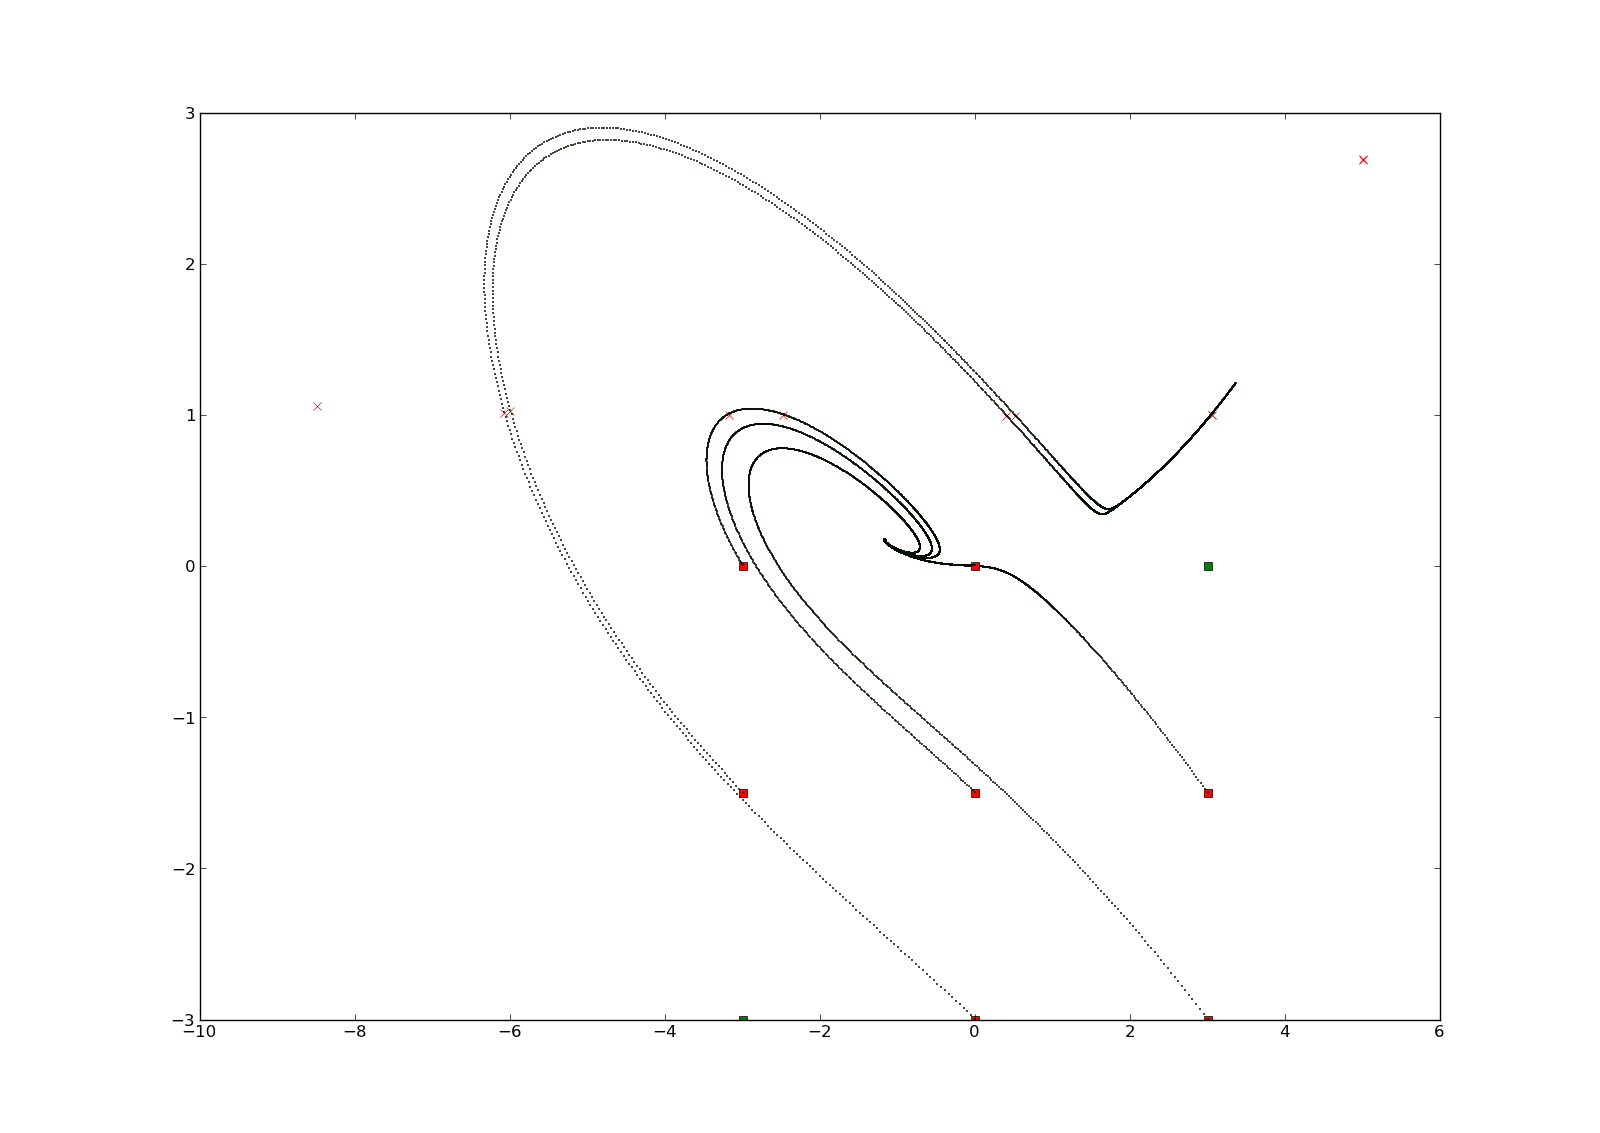
\includegraphics[scale=0.31,draft=false]{wh_reachability}
\label{fig:wh}
\caption{Reachability on Wilhelm Equations}
\end{figure}

\subsection*{Oscillation on Lotka-Volterra Equations}
Figure \ref{fig:lv} depicts $25$ seeds being examined for cycle presence
over an~$a\equiv x_1>5.4$ property. Black squares indicate seeds
for which no cycle is detected. Green squares are seeds for which
an oscillation formula
$\varphi\equiv\bG((a\implies\bF(\neg a))\wedge(\neg a\implies\bF(a)))$
holds. Red squares depict seeds for which a~cycle is detected but the
$\varphi$ formula does not hold. Red dots again represent filtered trace
points.

Due to accuracy of the integrator, 4\,000 numerical method
steps are taken to make the most of the seeds green and only the most
inner circle is a~true-negative. 

A~close-up of the situation can be seen in Figure \ref{fig:lv:close}.

\begin{figure}[h]
\center
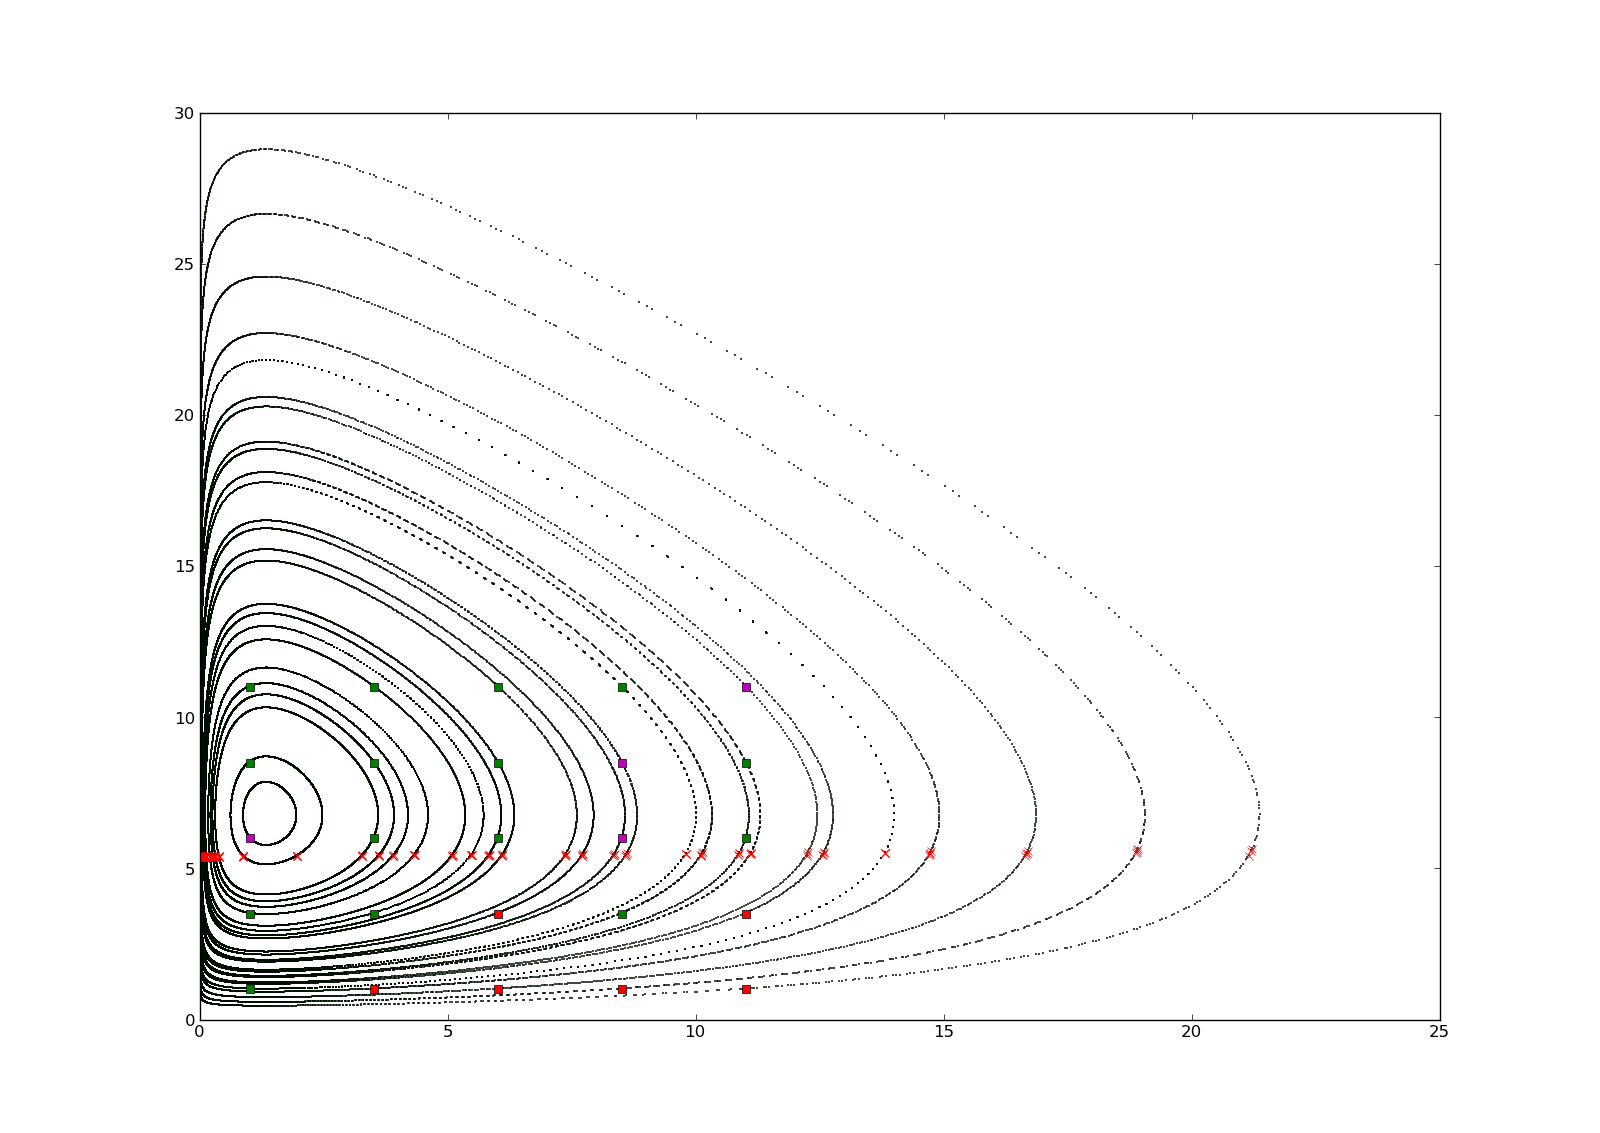
\includegraphics[scale=0.31,draft=false]{lv_oscillation}
\label{fig:lv}
\caption{Oscillation on Lotka-Volterra Equations}
\end{figure}

\begin{figure}[h]
\center
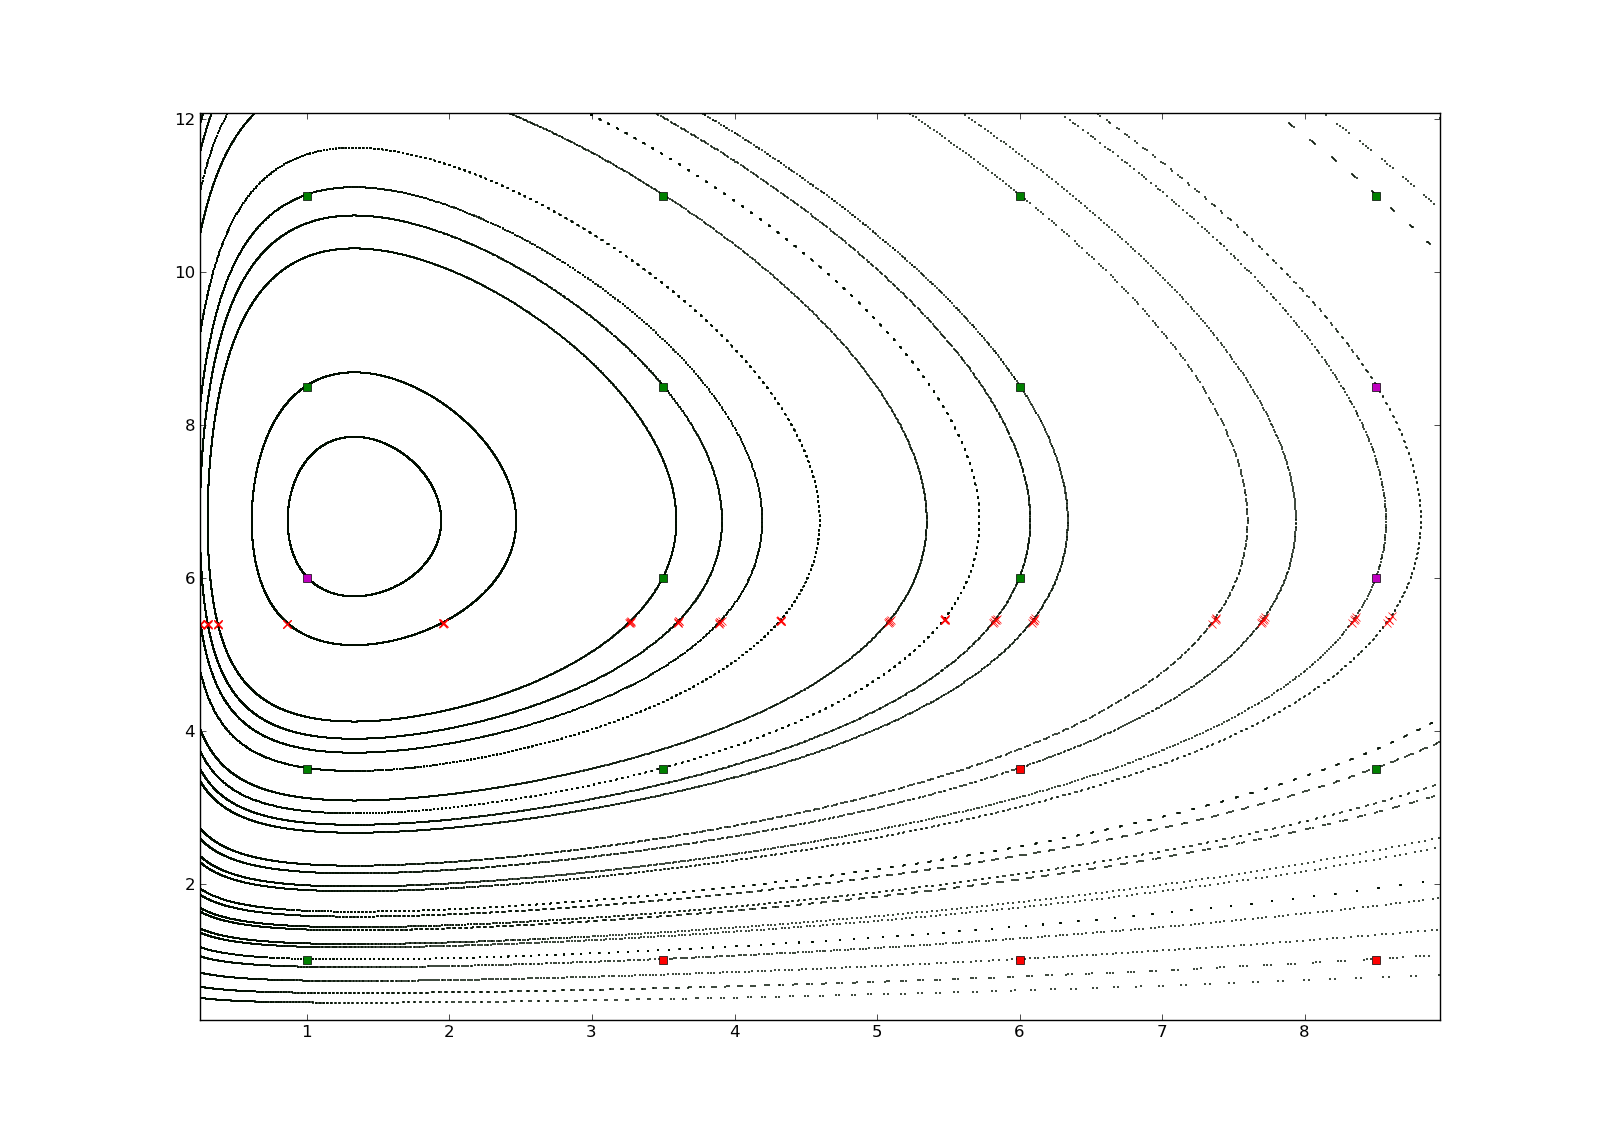
\includegraphics[scale=0.31,draft=false]{lv_oscillation_closeup}
\label{fig:lv:close}
\caption{Oscillation on Lotka-Volterra Equations\,--\,Close-up}
\end{figure}

\section{Performance}
If a~lasso-shaped or acyclic trace is considered, the number of steps
this method\,--\,including filtering and cycle detection\,--\,takes is
bound by $O(|AP|^2)$\cite{biere}.

When filtered, spiral traces after cycle detection of equilibrium point
contain $O(|AP|^d)$ elements, $d$ being the count of dimensions atomic
propositions refer to. This is because, unlike the loop, a~spiral trace
penetrates the constraints grid while converging to the equilibrium
point rather than encounter only the circumference constraints.
Therefore, the bound $k$ is of the same size. Together with the
sub-formula sharing, which is of quadratic complexity with regard to $k$,
the amount of steps for a~spiral trace is $O(|AP|^{2d})$ for the whole
method.

Altogether for deterministic system traces, the method takes only
polynomial amount of steps with regards to the atomic propositions
count as far as single trace is concerned.

\chapter{Future Work}
\section{Current Limitations}
Currently, the prototype has got following limitations:
\begin{inparaenum}[\itshape a\upshape)]
\item $\bU$ and $\bR$ operators are not implemented for cyclic model
	checking;
\item no parallelization for the model checking part is implemented;
\item experiments have got hard-coded settings;
\item custom-made partial derivations of each equation have to be
	provided for a~system to integrate;
\item the filtering does not yet work simultaneously with the numerical
	method;
\item poor accuracy integrator used;
\item no user interface; and
\item no native model description language support, such as
	\textsc{sbml}\cite{sbml}.
\end{inparaenum}

Removing these, a~more usable tool for analyzing the initial conditions
problem\cite{sven} or even for a~Monte Carlo based system robustness
analysis\cite{rizk} could be obtained.

\section{CUDA GPU Acceleration}
As imposed by the Algorithm \ref{simulationCycleDetectFilter}, the
filtering and cycle detection should cooperate together with the
numerical method. Therefore, an experimental \textsc{gpu} implementation
was started by the author\cite{me:cuda}. The project is based in
Papou\v{s}ek's thesis\cite{papousek} where a~numerical \textsc{gpu}
integration method is described. Papou\v{s}ek selected an approach of
one thread executing the integration algorithm for one dimension as this
assignment utilizes the \textsc{gpu} resources reasonably
well\cite{papousek}.

The same approach was selected by the author in \cite{me:cuda}; in the
filter, each trace examines the validity of an atomic proposition of
particular dimension. This happens after each\,``valid''\,numerical
method step and requires thread result synchronization for all the
computed point dimensions. Similarly, the cycle detection operates each
thread of a~warp comparing one dimension value of two points being
examined. Thus the filtering and cycle detection are suitable for
a~straightforward \textsc{gpu} parallelization.

However, the formula translation of the bounded model checking is
recursive and recursive functions are limited by some \textsc{cuda}
\textsc{api} versions\cite{cuda:relnotes}. Further limiting factor is
the need of sub-formula sharing during the translation process which
requires non-sequential memory access for a~hashing function to perform
optimally. Therefore, the Algorithm \ref{modelChecking} could be more
challenging task to implement on a~\textsc{gpu}.

Still, even if only the Algorithm \ref{simulationCycleDetectFilter}
is accelerated on \textsc{gpu}, the Algorithm \ref{modelChecking}
could be easily parallelized on \textsc{cpu} consuming output of the
filtered simulation effectively as it, too, does not require
synchronization amongst particular trace evaluations.

\chapter{Conclusion}
A prototype was created providing effective \ltl formula verification
for discrete time series of non-linear ordinary differential equation
systems or experimental data describing domain of population kinetics
of biological systems. Within the prototype, parts suitable for
\textsc{gpu} acceleration were identified, too.

The bounded model checking due to Biere et al.\,was utilized and
together with a~filtering method introduced here relaxed the computational
complexity of the model checking for these systems.

There remains not much to add now expect that the author sincerely hopes
there are readers for whom this work is useful.

\appendix
\chapter{Prototype Description}
The prototype is divided into python module files containing related classes.
For example, classes relevant for abstract expression manipulation are stored
in module \emph{ExpressionStructure}. In similar fashion, the rest of the
prototype is organized.

Each module has got a~short self-test section, thus if run, basic
functionality is checked.

\emph{Lotka-Volterra, Bayramov and Wilhelm} modules contain simulators of
particular dynamic systems. \emph{Brent and Sven} contain cycle detector
classes and \emph{Evaluation} modules provide cycle detection evaluation, when
run.

The \emph{Check}- modules provide property verification for particular system.
These are the reachability test of a~Wilhelm system in \emph{Check\_WH} and
oscillation over a~Lotka-Volterra system in \emph{Check\_LV} module.

The prototype was implemented and tested on a~\emph{Scientific Linux 6.1} and
a~\emph{Mac\,OS\,X~Snow\,Leopard} system in the
\emph{Enthought Python Distribution Free 7.2-1}.

The prototype utilizes \emph{Sci-Py} and \emph{NumPy} modules for graphical
representation, numerical integration and data storage.



\bibliographystyle{plainnat}
\bibliography{thesis}
\end{document}
\backmatter
